\begin{frame}{Objetivos}
	{Objetivo Geral}
		\begin{itemize}
		\item Elaborar e Aplicar um sistema automatizado de coleta, armazenamento e distribuição de água da chuva com base em uma cisterna pluvial;
	\end{itemize}
\end{frame}

\begin{frame}{Objetivos}
	{Objetivos Específicos}
	\begin{itemize}
		\item Elaborar um módulo denomiado \textbf{SMCC - Sistema de Medição e Controle da Cisterna} para aplicação no reservatório principal, realizando medições de nível, acionamento de \textit{motobomba}, direcionamento do fluxo de água e possuindo conexão com outros dispositivos via \textit{ Wi-Fi};
	\end{itemize}
\end{frame}

\begin{frame}{Objetivos}
	{Objetivos Específicos}
	\begin{itemize}
		\item Elaborar um módulo denominado \textbf{SMCCD - Sistema de Medição e Controle da Caixa D'água} para aplicação no reservatório auxiliar, realizando medições de nível, direcionamento do fluxo de água e possuindo conexão com outros dispositivos via \textit{Wi-Fi};
	\end{itemize}
\end{frame}

\begin{frame}{Objetivos}
	{Objetivos Específicos}
	\begin{itemize}
		\item Elaborar um aplicação \textit{Android Mobile} (denominada \textbf{SCCP APP}) e \textit{Desktop} (denominada \textbf{SCCP DESKTOP}) para executar as ações: ativação e desativação de uma bomba d'água, direcionamento do fluxo de água, visualização de dados provenientes de sensores e a possibilidade de definir as condições que executem rotinas de acionamento automático;
	\end{itemize}
\end{frame}

\begin{frame}{Objetivos}
	{Objetivos Específicos}
	\begin{itemize}
		\item Elaborar um sistema operacional embarcado conciso (baseado em \textit{kernel Linux}) aplicando-o a um microprocessador. O dispositivo deve possuir conexão com a \textit{Intranet} e servir como uma central de controle e armazenamento de dados, bem como ser hospedeiro do serviço de \textit{Broker MQTT};
	\end{itemize}
\end{frame}

\begin{frame}{Objetivos}
	{Objetivos Específicos}
	\begin{itemize}
		\item Incluir no sistema, rotinas de calibração para configurar os níveis e estados de operação em cisternas e caixas d'águas de tamanhos e formatos diferentes;
	\end{itemize}
\end{frame}

\begin{frame}{Objetivos}
	{Objetivos Específicos}
	\begin{itemize}
		\item Organizar um repositório \textit{online} para realização de futuros \textit{updates} ou \textit{upgrades} do \textit{firmware} embarcado;
	\end{itemize}
\end{frame}


\begin{frame}{Objetivos}
	{Objetivos Específicos}
	\begin{itemize}
		\item Planejar a implementação \textit{in loco},  analisando todos os fatores estruturais. Adqurir ou confeccionar instrumentos para proteção e suporte dos itens citados nos quesitos \textit{(a)} e \textit{(b)}.
	\end{itemize}
\end{frame}






\begin{frame}{Introdução}{Problema de Pesquisa}
	\vspace{-0.64cm}
	\begin{figure}[htp]
		\centering
		\caption{\centering{\small{Sistema legado de iluminação e medição de energia predial}}}
		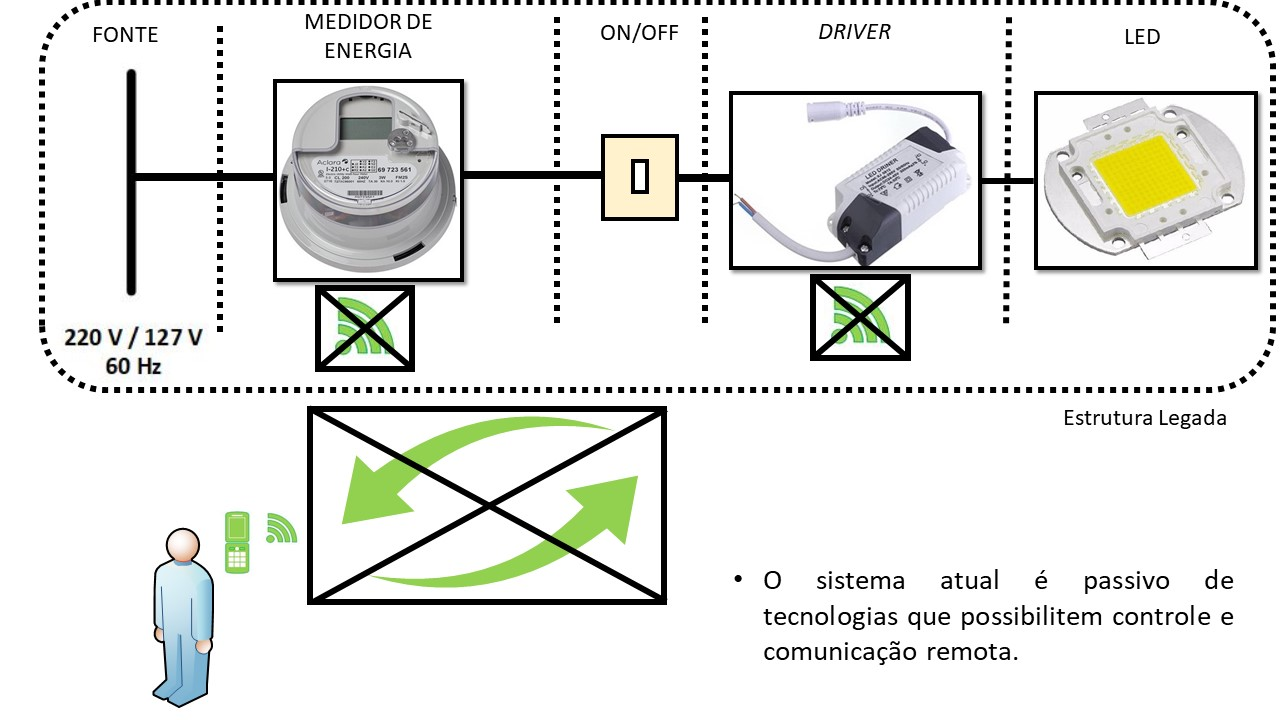
\includegraphics[width=0.97\linewidth]{img/1.jpg}
		\hspace{5cm}
		\vspace{5cm}
		\legend{\small{Fonte: Adaptado \cite{gomes,fernandes2018implementation,medidor}}}
	\end{figure}
	
\end{frame}

\begin{frame}{Introdução}{Problema de Pesquisa}
	\vspace{-0.64cm}
	\begin{figure}[htp]
		\centering
		\caption{\centering{\small{Uma alternativa a convergência \textit{Smart Building}}}}
		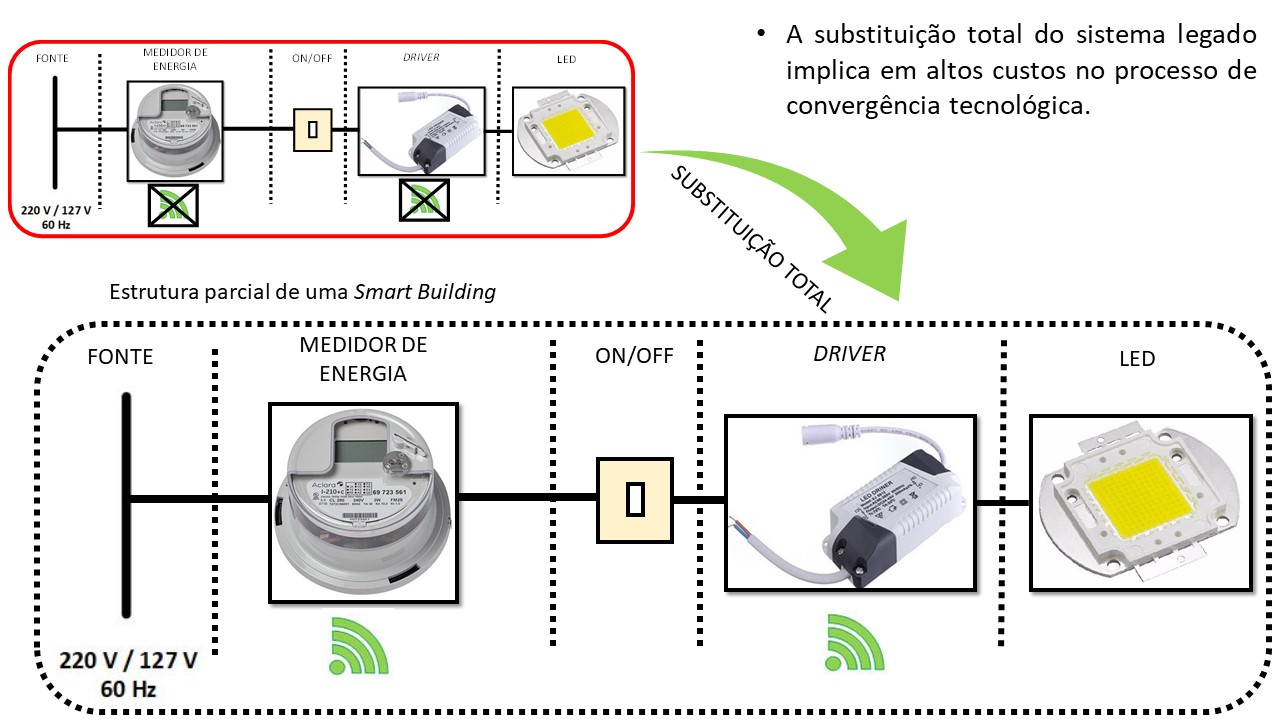
\includegraphics[width=0.97\linewidth]{img/2.jpg}
		\hspace{5cm}
		\vspace{5cm}
		\legend{\small{Fonte: Adaptado \cite{gomes,fernandes2018implementation,medidor}}}
	\end{figure}
	
\end{frame}


\begin{frame}{Introdução}{Problema de Pesquisa}
	\vspace{-0.64cm}
	\begin{figure}[htp]
		\centering
		\caption{\centering{\small{Como efetuar a convergência \textit{Smart Building}?}}}
		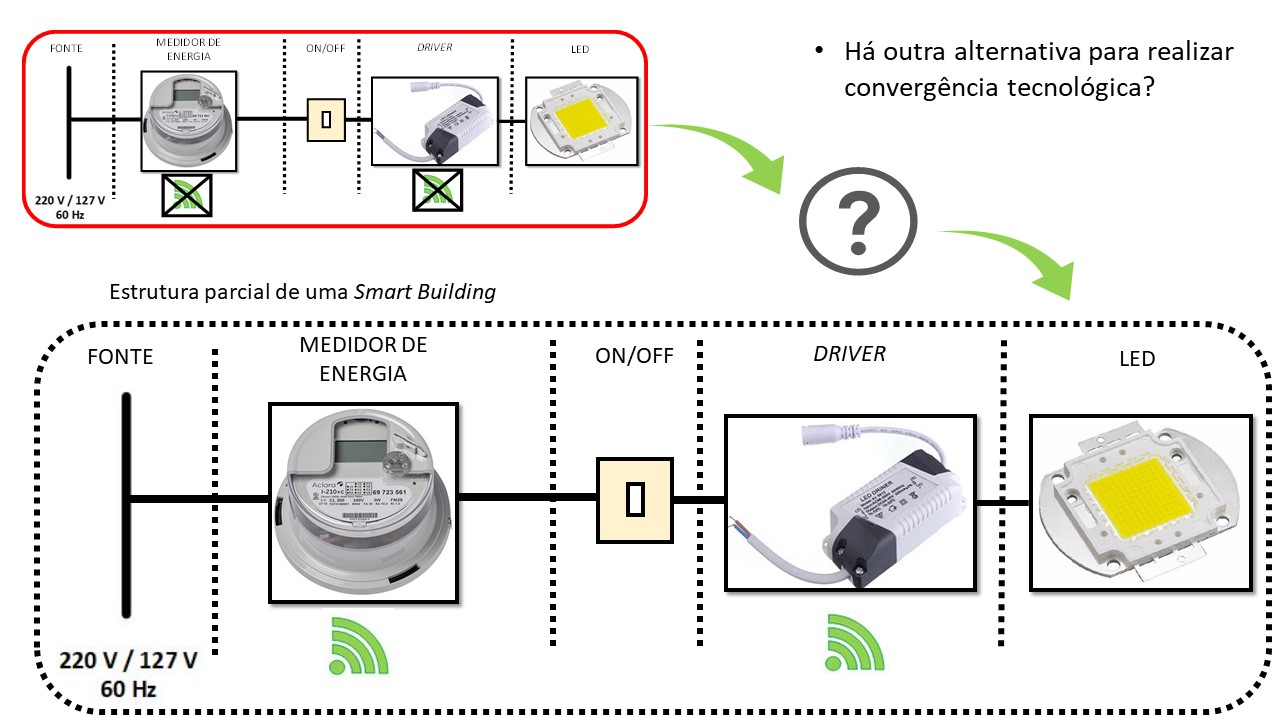
\includegraphics[width=0.97\linewidth]{img/3.jpg}
		\hspace{5cm}
		\vspace{5cm}
		\legend{\small{Fonte: Adaptado \cite{gomes,fernandes2018implementation,medidor}}}
	\end{figure}
	
\end{frame}


\begin{frame}{Introdução}{Hipótese}
	\vspace{-0.64cm}
	\begin{figure}[htp]
		\centering
		\caption{\centering{\small{A estratégia do \textit{retrofit}}}}
		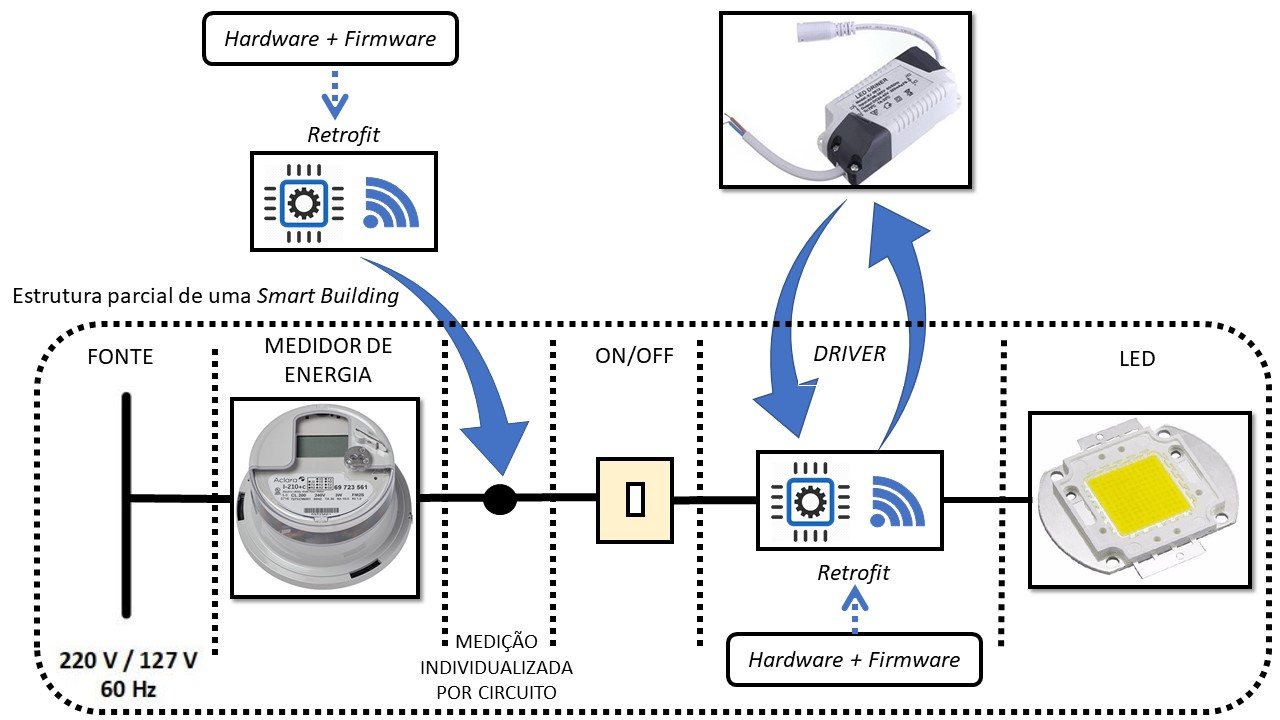
\includegraphics[width=0.97\linewidth]{img/4.jpg}
		\hspace{5cm}
		\vspace{5cm}
		\legend{\small{Fonte: Adaptado \cite{gomes,fernandes2018implementation,medidor}}}
	\end{figure}
	
\end{frame}


\begin{frame}{Introdução}{Hipótese}
	\vspace{-0.64cm}
	\begin{figure}[htp]
		\centering
		\caption{\centering{\small{O \textit{retrofit} associado a plataforma SmartLVGrid para realizar a convergência \textit{Smart Building}}}}
		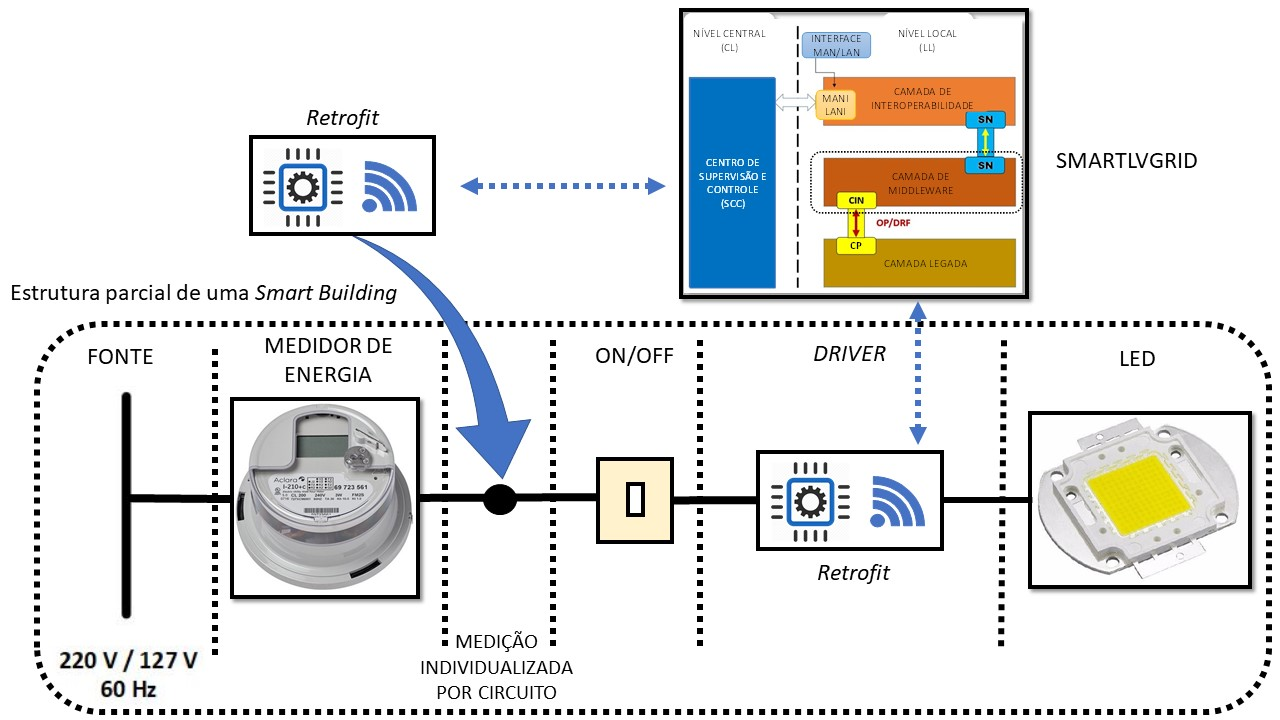
\includegraphics[width=0.915\linewidth]{img/5.jpg}
		\hspace{5cm}
		\vspace{5cm}
		\legend{\small{Fonte: Adaptado \cite{gomes,fernandes2018implementation,medidor}}}
	\end{figure}
	
\end{frame}

\begin{frame}{Introdução}{Justificativas}
	\vspace{-0.64cm}
	\begin{figure}[htp]
		\centering
		\caption{\centering{\small{Justificativas do projeto}}}
		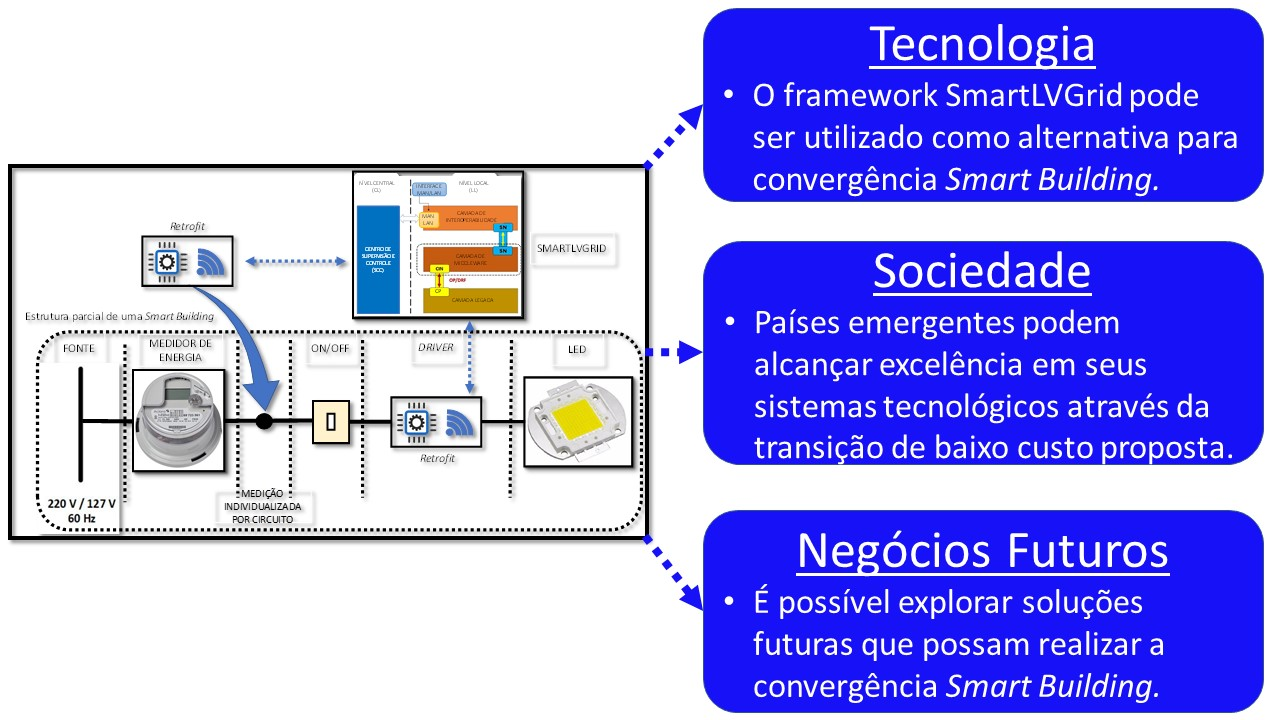
\includegraphics[width=0.97\linewidth]{img/6.jpg}
		\hspace{5cm}
		\vspace{5cm}
		\legend{\small{Fonte: Adaptado \cite{gomes,fernandes2018implementation,medidor}}}
	\end{figure}
	
\end{frame}

\begin{frame}{Introdução}{Objetivos}
	\begin{block}{Objetivo Geral}
		\justify{\small{Desenvolver plataformas de \textit{hardware} e\textit{ firmware}, a camada de
				\textit{middleware} do \textit{framework} SmartLVGrid, aplicadas ao retrofit de luminárias LED e de circuitos
				de medição de energia elétrica, de forma a viabilizar a convergência \textit{smart building} de circuitos elétricos e iluminação de ambientes e melhorar a eficiência energética.}}
	\end{block}
	
	\begin{block}{Objetivos Específicos}
		\begin{itemize}
			\small{	\item definir contornos conceituais do \textit{framework} SmartLVGrid e do paradigma \textit{smart building};
				\item estudar soluções para controle de sistemas de iluminação LED e para telemedição de parâmetros elétricos;
				\item projetar e implementar módulos embarcados de \textit{retrofit} de acordo com o \textit{framework} SmartLVGrid;
				\item realizar análises dos resultados obtidos no processo de convergência \textit{smart building} com o uso do SmartLVGrid.}
		\end{itemize}
	\end{block}
\end{frame}

